\chapter{meltovision}
\label{sec:meltovision}
\lstset{style=68KStyle}
\lhead[tempest 2000]{}
'melt-o-vision' was the name given to a neat interstitial feature in Tempest 2000 where
the screen blurs, rotates and fades before transitioning to the next screen.

\begin{figure}[H]
    \centering
    \centerline{\frame{\includegraphics[width=5.5cm]{src/meltovision/1.png}}%
    \hspace{0.2cm}
    \frame{\includegraphics[width=5.5cm]{src/meltovision/2.png}}}%
    \vspace{0.2cm}
    \centerline{\frame{\includegraphics[width=5.5cm]{src/meltovision/3.png}}%
    \hspace{0.2cm}
    \frame{\includegraphics[width=5.5cm]{src/meltovision/4.png}}}%
  \caption{Melt-o-vision in action.}
\end{figure}

\begin{lstlisting}
; *******************************************************************
; fade ; Do a meltovision transition.
; This is meltovision.
; https://www.trademarkia.com/meltovision-74534584
; Go into FADE after merging screen3 to current screen and
; turning off BEASTIES+64
; *******************************************************************
fade:   tst beasties+76            ; Are we ready for meltovision?
        bmi ofade                  ; If so, do a meltovision transition.
        ; If not do a merge first.
        move.l #screen3,a0         ; Point a0 at screen3.
        move.l gpu_screen,a1       ; Point a1 at gpu_screen.
        moveq #0,d0                ; X position in source screen
        moveq #0,d1                ; Y position in source screen
        move #384,d2               ; Width
        move #240,d3               ; Height
        add palfix1,d3             ; Adjust for PAL
        moveq #0,d4                ; X position in destination screen.
        moveq #0,d5                ; Y position in destination screen.
        tst mfudj                  ; Fudging height required?
        beq pmf2                   ; If not, skip.
        sub #8,d3                  ; Otherwise fudge source height by 8.
    
pmfade: tst mfudj                  ; Fudging height required?
        beq pmf2                   ; If not, skip.
        add #8,d5                  ; Otherwise fudge dest height by 8.
        clr mfudj                  ; Clear the fudge factor.

        ; Now we can merge the two screens together. 
pmf2:   jsr MergeBlock             ; Merge screen3 and gpu_screen
        move #-1,beasties+76       ; Signal we can do a fade now.
    
        ; Now we can set up melt-o-vision (tm).
ofade:  clr _pauen                 ; Can't pause in fade
        move.l #ffade,demo_routine ; Set meltovision as the demo_routine
        move.l #failcount,routine  ; Set the counter routine.
        move #150,pongx            ; Set the x counter to 150
        ; Get a random value for pongz.
        jsr rannum                 ; Random number between 0 and 255 in d0.
        and #$7,d0                 ; Just the last 3 bits please.
        sub #$03,d0                ; Subtract 3.
        and #$ff,d0                ; Keep the result between 0 and 255
        move d0,pongz              ; Set as pongz (our z counter).
        move.l #$f80000,delta_i    ; Set our delta intensity.
        move z,-(a7)               ; Stash z in the stack.
        clr z                      ; Clear hard reset signal.
        bsr gogame                 ; Run the meltovision transition.
        move.l #screen3,a0         ; Point a0 at screen3.
        jsr clrscreen              ; Clear the screen in a0.
        move (a7)+,z               ; Restore z from the stack.
        move #1,sync               ; Signal a sync is required.
        rts
\end{lstlisting}
\clearpage

This innovation was so important Atari decide to trademark it. They later decided it
wasn't important at all and abandoned the trademark. That's how business works I guess. 

In order to scale, rotate and zoom the current screen we need to merge the two layers its
composed of. This means taking \icode{gpu\_screen}, which is the 'background', and \icode{screen3},
which is our 'foreground', and compositing them so we have one region of data we can manipulate. 

\begin{figure}[H]
  {
    \setlength{\tabcolsep}{3.0pt}
    \setlength\cmidrulewidth{\heavyrulewidth} % Make cmidrule = 
    \begin{adjustbox}{center}
      \begin{tabular}[t]{lll}
        \toprule
        Raw Data & Parsed Data & Image at \icode{gpu\_screen} (\icode{0x100000}) \\
        \midrule
          \tcode{10,00,00,1D,6E,45,C1,60}
        &
        \makecell[tl]{
          \begingroup
          \renewcommand{\arraystretch}{.8} % Default value: 1
          \begin{tabular}[t]{ll}
            \tcode{TYPE: 0}   &    \tcode{LINK: 0xeb70}  \\
            \tcode{YPOS: 44} &     \tcode{DATA: 0x100000}  \\
            \tcode{HEIGHT: 279} &  \\
            \tcode{} &  \\
            \tcode{} &  \\
          \end{tabular}
          \endgroup
        } &
        \multirow{2}{*}[0.1cm]{
          \makecell[tl]{
            \includegraphics[height=4.2cm]{object_list/data_1_hiscore.png}%
          }
        } \\
        \addlinespace
          \tcode{00,00,80,06,01,80,CF,F8}
        &
        \makecell[tl]{
          \begingroup
          \renewcommand{\arraystretch}{.8} % Default value: 1
          \begin{tabular}[t]{ll}
            \tcode{XPOS: -7   } &  \tcode{REFLECT: 0}  \\
            \tcode{DEPTH: 4} &    \tcode{RMW: 0}  \\
            \tcode{PITCH: 1} &    \tcode{TRANS: 1}  \\
            \tcode{DWIDTH: 96} &  \tcode{RELEASE: 0}  \\
            \tcode{IWIDTH: 96} &  \tcode{FIRSTPIX: 0}  \\
            \tcode{INDEX: 0} & \\
          \end{tabular}
          \endgroup
        } &
        \\
        \midrule
        Raw Data & Parsed Data & Image at \icode{screen3} (\icode{0x50000}) \\
        \midrule
          \tcode{05,00,00,1D,72,45,C1,60}
        &
        \makecell[tl]{
          \begingroup
          \renewcommand{\arraystretch}{.8} % Default value: 1
          \begin{tabular}[t]{ll}
            \tcode{TYPE: 0}   &    \tcode{LINK: 0xeb90}  \\
            \tcode{YPOS: 44} &     \tcode{DATA: 0x50000}  \\
            \tcode{HEIGHT: 279} &  \\
            \tcode{} &  \\
            \tcode{} &  \\
          \end{tabular}
          \endgroup
        } &
        \multirow{2}{*}[0.1cm]{
          \makecell[tl]{
            \includegraphics[height=4.2cm]{object_list/data_4_hiscore.png}%
          }
        } \\
        \addlinespace
          \tcode{00,00,80,06,01,80,CF,F8}
        &
        \makecell[tl]{
          \begingroup
          \renewcommand{\arraystretch}{.8} % Default value: 1
          \begin{tabular}[t]{ll}
            \tcode{XPOS: -7   } &  \tcode{REFLECT: 0}  \\
            \tcode{DEPTH: 4} &    \tcode{RMW: 0}  \\
            \tcode{PITCH: 1} &    \tcode{TRANS: 1}  \\
            \tcode{DWIDTH: 96} &  \tcode{RELEASE: 0}  \\
            \tcode{IWIDTH: 96} &  \tcode{FIRSTPIX: 0}  \\
            \tcode{INDEX: 0} & \\
          \end{tabular}
          \endgroup
        } &
        \\
        \bottomrule
      \end{tabular}
    \end{adjustbox}
  }
\end{figure}

We do all of this in the \icode{fade} routine on the opposite page. Once we have our source
and destination co-ordinates ready we can call \icode{MergeBlock} to do the compositing:

\begin{lstlisting}
        ; Now we can merge the two screens together. 
pmf2:   jsr MergeBlock             ; Merge screen3 and gpu_screen
\end{lstlisting}

\icode{MergeBlock}, which we reproduce on the next page, consists of a call to the Jaguar's
'Blitter' with a simple command to draw the contents of \icode{screen3} onto \icode{gpu\_screen}.
\clearpage
\begin{lstlisting}
MergeBlock:
        move.l #0,B_PATD   ; Set transparency colour.
        move.l #0,B_PATD+4 ; Set transparency colour
    
        ; Set up the blitter command.
        move.l #PITCH1|PIXEL16|WID384|XADDINC,d7
        move.l d7,A1_FLAGS ; Set the Source screen flags.
    
        move.l #PITCH1|PIXEL16|WID384|XADDPIX|YADD1,d7
        move.l d7,A2_FLAGS ; Set the Dest screenf lags.
    
        ; d3 is the height, d2 is the width.
        move d3,d7         ; Put d3 (height) in lower word of d7.
        swap d7            ; Swap position of first 2 bytes with last 2.
        move d2,d7         ; Put d2 (width) in lower word of d7.
        move.l d7,B_COUNT  ; Store as inner and outer loop counts
    
        ; Set up the origin of source screen (x:d0, y:d1). 
        move d1,d7         ; Put d1 (Y pos) in lower word of d7.
        swap d7            ; Swap position of first 2 bytes with last 2.
        move d0,d7         ; Put d0 (X pos) in lower word of d7.
        move.l d7,A1_PIXEL ; Store as X and Y origin of source screen.
    
        ; Set up the origin of dest screen (x:d4, y:d5). 
        move d5,d7         ; Put d5 (Y pos) in lower word of d7.
        swap d7            ; Swap position of first 2 bytes with last 2.
        move d4,d7         ; Put d4 (X pos) in lower word of d7.
        move.l d7,A2_PIXEL ; Store as X and Y origin of dest screen.
    
        move.l #0,A1_FPIXEL
        move.l #$0001,A1_INC
        move.l #$0,A1_FINC
    
        ; Set our width (d2) as the number of loop steps.
        move #1,d7         ; Store 1 in d7
        swap d7            ; Swap position of first 2 bytes with last 2.
        move d2,d7         ; Put d2 (width) in lower word of d7.
        neg d7             ; Make it negative.
        move.l d7,A1_STEP  ; Store as the number of loops for source.
        move.l d7,A2_STEP  ; Store as the number of loops for dest.
    
        ; Copy the screen data for source and dest.
        move.l a0,d7       ; Copy the source screen (a0) to d7.
        move.l d7,A1_BASE  ; Set it as our source screen.
        move.l a1,d7       ; Copy the destination (a1) to d7.
        move.l d7,A2_BASE  ; Set it as our destination screen.
    
        ; Run the blitter command to draw one block onto the other.
        move.l #SRCEN|UPDA1|UPDA2|DSTA2|LFU_A|LFU_AN|DCOMPEN,d7
        move.l d7,B_CMD    ; Run the blitter command.
        bra WaitBlit       ; Wait for the blitter to finish.
\end{lstlisting}
\clearpage
The result is we go from having an object list with two screens, to just one, containing the
\icode{gpu\_screen}. Here is what the object list contains with the two screens merged
and the melt-o-vision transition from the high score screen just getting started.

\begin{figure}[H]
  {
    \setlength{\tabcolsep}{3.0pt}
    \setlength\cmidrulewidth{\heavyrulewidth} % Make cmidrule = 
    \begin{adjustbox}{center}
      \begin{tabular}[t]{lll}
        \toprule
        Raw Data & Parsed Data & Image at \icode{gpu\_screen} (\icode{0x100000}) \\
        \midrule
          \tcode{10,00,00,1D,6E,45,C1,60}
        &
        \makecell[tl]{
          \begingroup
          \renewcommand{\arraystretch}{.8} % Default value: 1
          \begin{tabular}[t]{ll}
            \tcode{TYPE: 0}   &    \tcode{LINK: 0xeb70}  \\
            \tcode{YPOS: 44} &     \tcode{DATA: 0x100000}  \\
            \tcode{HEIGHT: 279} &  \\
            \tcode{} &  \\
            \tcode{} &  \\
          \end{tabular}
          \endgroup
        } &
        \multirow{2}{*}[0.1cm]{
          \makecell[tl]{
            \includegraphics[height=4.2cm]{meltovision/data_1.png}%
          }
        } \\
        \addlinespace
          \tcode{00,00,80,06,01,80,CF,F8}
        &
        \makecell[tl]{
          \begingroup
          \renewcommand{\arraystretch}{.8} % Default value: 1
          \begin{tabular}[t]{ll}
            \tcode{XPOS: 4088} &  \tcode{REFLECT: 0}  \\
            \tcode{DEPTH: 4} &    \tcode{RMW: 0}  \\
            \tcode{PITCH: 1} &    \tcode{TRANS: 1}  \\
            \tcode{DWIDTH: 96} &  \tcode{RELEASE: 0}  \\
            \tcode{IWIDTH: 96} &  \tcode{FIRSTPIX: 0}  \\
            \tcode{INDEX: 0} & \\
          \end{tabular}
          \endgroup
        } &
        \\
        \bottomrule
      \end{tabular}
    \end{adjustbox}
  }
\end{figure}

Going back to the \icode{fade} routine we can see that the next step after merging
the two screens is to set up the meltovision transition itself. This consists of
setting our GPU manager routine to \icode{ffade} and a co-routine \icode{failcount}
that will track our progress along the X axis:

\begin{lstlisting}
    move.l #ffade,demo_routine ; Set meltovision as the demo_routine
    move.l #failcount,routine  ; Co-routine to bail when pongx reaches 0.
\end{lstlisting}
And determining how much movement along the X axis (\icode{pongx}) and how much rotation around the Z
axis (\icode{pongz}) the transition will consist of:
\begin{lstlisting}
    move #150,pongx            ; Set the x counter to 150
    ; Get a random value for pongz.
    jsr rannum                 ; Random number between 0 and 255 in d0.
    and #$7,d0                 ; Just the last 3 bits please.
    sub #$03,d0                ; Subtract 3.
    and #$ff,d0                ; Keep the result between 0 and 255
    move d0,pongz              ; Set as pongz (our z counter).
\end{lstlisting}

Notice that we keep our rotation step (which is really an angle value) between 0 and 7, i.e. just
the last 3 bits.
With this done we can start running the meltovision transition itself:

\begin{lstlisting}
    bsr gogame                 ; Run the meltovision transition.
\end{lstlisting}
\icode{gogame}, which we won't print here, simply runs in a loop and invokes \icode{ffade}
until \icode{failcount} has reduced \icode{pongx} to zero.
\clearpage
\begin{lstlisting}
ffade:
        ; This section ensures we only rotate a little, i.e. 7
        ; individual rotations of our value in pongz.
        add #1,pongy          ; Increment pongy.
        move pongy,d0         ; Move it to d0.
        and #$03,d0           ; Select the lowest 3 bits only.
        bne failfade          ; If non-zero, do a step in meltovision.
        tst.b pongz+1         ; Check pongz (out angle of rotation)..
        beq failfade          ; If it's zero, do a meltovision step.
        bmi ffinc             ; If it's negative, increment it.
        sub.b #2,pongz+1      ; Otherwise decrement it by 2.
ffinc:  add.b #1,pongz+1      ; Increment pongz.

        ; Run a step in the meltovision transition.
failfade:
        move.l #(PITCH1|PIXEL16|WID384),d0 ; Set d0 with our flags.
        move.l d0,source_flags ; Set as the source flags.
        move.l d0,dest_flags  ; And set as the dest flags.
        lea in_buf,a0         ; Point our GPU RAM input buffer at a0.
        move pongz,d0         ; Put angle of rotation in d0.
        and.l #$ff,d0         ; Keep it between 0 and 255
        move.l cscreen,(a0)   ; Put source screen in GPU buffer.
        move.l #384,4(a0)     ; Store full-screen width in GPU buffer.
        move.l #240,d1        ; Store full-screen height in d1.
        add palfix1,d1        ; Adjust for PAL screens if required.
        move.l d1,8(a0)       ; Store height in buffer.
        move.l #$1f4,12(a0)   ; Put X scale in GPU buffer.
        move.l #$1f4,16(a0)   ; Put Y scale in GPU buffer.
        move.l d0,20(a0)      ; Put initial angle in brads in GPU buffer.
        move.l #$c00000,24(a0); source x centre in 16:16
        move.l #$780000,d0    ; Set inital y centre position.
        add.l palfix3,d0      ; Adjust for PAL screens if required.
        move.l d0,28(a0)      ; Put y centre in GPU buffer.
        move.l #$0,32(a0)     ; offset of dest rectangle
        move.l delta_i,36(a0) ; change of i per increment
        ; Select 'scar' in antelope.gas.
        ; Op 2 of this module is Scale and Rotate
        move.l #2,gpu_mode    ; Select 'scar' in antelope.gas
        move.l #demons,a0     ; Load the demons module (antelope.gas).
        jsr gpurun            ; Run it.
        jmp gpuwait           ; Wait until GPU finished.
\end{lstlisting}
\begin{lstlisting}
failcount:
        sub #1,pongx         ; Subtract 1 from pongx.
        bpl rrrts            ; If still positive we're not done yet.
        move #-1,x_end       ; Signal we're done
        move #1,screen_ready ; Signal screen ready for display.
        rts
\end{lstlisting}
\clearpage
 We can play with a few parameters to alter the effect, and this will help us understand how it works.
 
 For example, if we change our angle of rotation for each step to -16, by changing the following
 line in \icode{fade} from:
\begin{lstlisting}
        move d0,pongz          ; Store d0 in pongz.
\end{lstlisting}
to:
\begin{lstlisting}
        move #$f0,pongz        ; Store -16 in pongz.
\end{lstlisting}
And if we increase the number of allowed rotations from 7 (3 bits) in \icode{ffade} (opposite) from:
\begin{lstlisting}
        and #$03,d0           ; Select the lowest 3 bits only.
\end{lstlisting}
to 256 (8 bits):
\begin{lstlisting}
        and #$ff,d0           ; Select the whole byte instead.
\end{lstlisting}

We get an entertainingly rapid rotation of the screen!
\begin{figure}[H]
    \centering
    \centerline{\frame{\includegraphics[width=4cm]{src/meltovision/rotate/1.png}}%
      \hspace{0.2cm}
      \frame{\includegraphics[width=4cm]{src/meltovision/rotate/2.png}}%
      \hspace{0.2cm}
      \frame{\includegraphics[width=4cm]{src/meltovision/rotate/3.png}}}%
    \vspace{0.2cm}
    \centerline{\frame{\includegraphics[width=4cm]{src/meltovision/rotate/4.png}}%
      \hspace{0.2cm}
      \frame{\includegraphics[width=4cm]{src/meltovision/rotate/5.png}}%
      \hspace{0.2cm}
      \frame{\includegraphics[width=4cm]{src/meltovision/rotate/6.png}}}%
  \caption{Melt-o-vision with a faster rotation.}
\end{figure}

We can also get rid of the rotation completely and alter the scaling factor to see
what happens. Let's do that:

\begin{minipage}[c]{0.48\linewidth}
\begin{lstlisting}[basicstyle=\scriptsize\ttfamily]
move pongz,d0         ; Initial angle.

..
move.l #$1f4,12(a0)   ; X scale.
move.l #$1f4,16(a0)   ; Y scale.
\end{lstlisting}
\end{minipage}
\hspace{0.1cm}
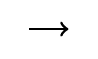
\begin{tikzpicture}
  \draw[->,line width=1pt] (0,0) to (0.5,0);
\end{tikzpicture}
\hspace{0.1cm}
\begin{minipage}[c]{0.48\linewidth}
\begin{lstlisting}[basicstyle=\scriptsize\ttfamily]
move #$00,d0         ; No rotation.
nop
..
move.l #$208,12(a0)  ; X scale.
move.l #$208,16(a0)  ; Y scale.
\end{lstlisting}
\vspace*{\fill}
\end{minipage}

We've increased the scaling factor from \icode{\$1f4} to \icode{\$208}. The results are 
slightly strange.
\begin{figure}[H]
    \centering
    \centerline{\frame{\includegraphics[width=4cm]{src/meltovision/scale/1.png}}%
      \hspace{0.2cm}
      \frame{\includegraphics[width=4cm]{src/meltovision/scale/3.png}}%
      \hspace{0.2cm}
      \frame{\includegraphics[width=4cm]{src/meltovision/scale/5.png}}}%
    \vspace{0.2cm}
    \centerline{\frame{\includegraphics[width=4cm]{src/meltovision/scale/7.png}}%
      \hspace{0.2cm}
      \frame{\includegraphics[width=4cm]{src/meltovision/scale/9.png}}%
      \hspace{0.2cm}
      \frame{\includegraphics[width=4cm]{src/meltovision/scale/11.png}}}%
  \caption{Melt-o-vision with a higher scale factor and no rotation.}
\end{figure}

We get no obvious scaling of the image anymore, except across the central X/Y axis.

If we play with the centre Y position, by increasing it, we observe a different effect.

\begin{minipage}[c]{0.48\linewidth}
\begin{lstlisting}[basicstyle=\scriptsize\ttfamily]
move pongz,d0         ; Initial angle.

..
move.l #$780000,d0    ; Initial Y centre.
\end{lstlisting}
\end{minipage}
\hspace{0.1cm}
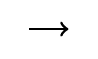
\begin{tikzpicture}
  \draw[->,line width=1pt] (0,0) to (0.5,0);
\end{tikzpicture}
\hspace{0.1cm}
\begin{minipage}[c]{0.48\linewidth}
\begin{lstlisting}[basicstyle=\scriptsize\ttfamily]
move #$00,d0         ; No rotation.
nop
..
move.l #$7F0000,d0    ; Initial Y centre.
\end{lstlisting}
\vspace*{\fill}
\end{minipage}

With a 'center' north of the centre of the screen the scaling ascends out of the
top of the screen.
\begin{figure}[H]
    \centering
    \centerline{\frame{\includegraphics[width=4cm]{src/meltovision/center/1.png}}%
      \hspace{0.2cm}
      \frame{\includegraphics[width=4cm]{src/meltovision/center/3.png}}%
      \hspace{0.2cm}
      \frame{\includegraphics[width=4cm]{src/meltovision/center/5.png}}}%
    \vspace{0.2cm}
    \centerline{\frame{\includegraphics[width=4cm]{src/meltovision/center/7.png}}%
      \hspace{0.2cm}
      \frame{\includegraphics[width=4cm]{src/meltovision/center/9.png}}%
      \hspace{0.2cm}
      \frame{\includegraphics[width=4cm]{src/meltovision/center/10.png}}}%
  \caption{Melt-o-vision with a higher center factor and no rotation.}
\end{figure}

